\chapter{Introduzione alle Tecnologie del Linguaggio Naturale}

\section{Prologo}

La prima parte del corso sarà incentrata sulla linguistica computazionale generale, in cui ci si soffermerà sugli aspetti più tradizionali e linguistici\footnote{Libro di riferimento: An Introduction to Natural Language Processing,
Computational Linguistics, and Speech Recognition. La prima e la seconda edizione, perché Jurafsky non riesce a finire il draft della terza :(}. In questa parte verrà anche trattato il parsing. Nella seconda parte si andranno a studiare la semantica lessicale e le ontologie. Infine, nella terza parte del corso si andrà a studiare NLP statistico e distribuzionale.

\begin{figure}[h]
    \centering
    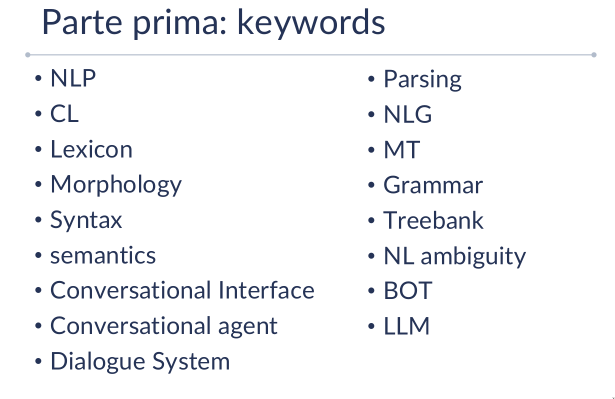
\includegraphics[scale=0.75]{01/key.png}
    \caption{Il giorno prima dell'esame bisogna sapere cosa significano tutte queste parole :3}
\end{figure}

\paragraph{Le 4 ere della linguistica computazionale:}

\begin{enumerate}
  \item 1940 - 1969: primi tentativi. 
  \item 1970 - 1992: formalizzazione. 
  \item 1993 - 2012: apprendimento automatico. 
  \item 2013 - 2018: deep learning.
\end{enumerate}

\nt{Tutto cambiò nel 2018, quando NLP fu il primo successo su larga scala di rete neurale autosupervisionata.}

\begin{figure}[h]
    \centering
    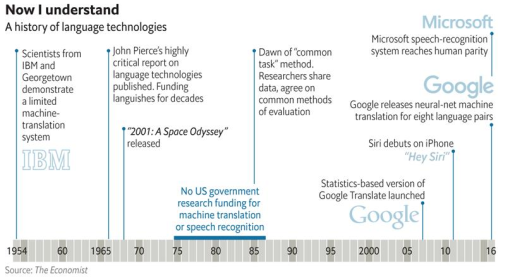
\includegraphics[scale=0.75]{01/timeline.png}
    \caption{Il passato delle tecnologie del linguaggio naturale.}
\end{figure}

\subsection{La Complessità del Linguaggio Naturale}

C'è un legame tra linguaggio umano e intelligenza. Già Turing sosteneva che se si potesse parlare in un certo modo si fosse intelligenti (test di Turing). La differenza tra il linguaggio umano e un linguaggio di programmazione è l'\fancyglitter{ambiguità}: C o Java non sono ambigui.

\paragraph{Il linguaggio umano:}

\begin{itemize}
  \item \fancyglitter{Discretezza} (esistenza di elementi): 
    \begin{itemize}
      \item Api: Ritmo, orientamento, durata. 
      \item Esseri umani: Fonemi, morfemi, parole.
    \end{itemize}
  \item \fancyglitter{Ricorsività}: 
    \begin{itemize}
      \item Scimpanze: Gesti atomici. 
      \item Uomo: Gianni vede Pietro, Maria vuole che Gianni veda Pietro, Paolo crede che Maria voglia che Gianni veda Pietro.
    \end{itemize}
  \item \fancyglitter{Dipendenza dalla struttura}: 
    \begin{itemize}
      \item Non “una parola dietro l'altra” ma c'è una struttura: La ragazza parte, I ragazzi di cui mi ha parlato la ragazza partono. 
    \end{itemize}
  \item \fancyglitter{Località}: 
    \begin{itemize}
      \item Gianni lo ha guardato. 
      \item Gianni ha detto che Pietro lo ha guardato.
    \end{itemize}
\end{itemize}

\paragraph{Intelligenza e linguaggio nel il test di Turing:}

\begin{itemize}
  \item Possono le macchine pensare?
  \item Se riesco a parlare come un essere umano allora penso. 
  \item Gioco dell'imitazione: un giudice deve capire se quello che ha davanti è un uomo oppure un computer.
\end{itemize}

\nt{Ci sono una serie di obiezioni a questo test: teologia, matematica, coscienza, etc.}

\begin{figure}[h]
    \centering
    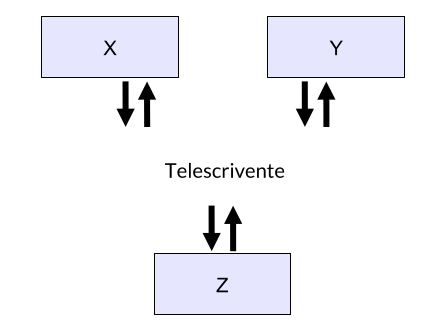
\includegraphics[scale=0.6]{01/Turing.png}
    \caption{Il gioco dell'imitazione.}
\end{figure}

\subsubsection{}

Nel 1966, Weizenbaum crea Eliza. Una macchina in grado di "comprendere" e ingannare gli esseri umani.

\nt{Il punto debole del test di Turing e di Eliza è il giudice: se è coinvolto emotivamente potrebbe far passare un computer per un essere umano\footnote{Blade runner moment}.}

\dfn{Winograd Schema}{
  Evoluzione del Turing test: un test a scelta multipla che utilizza domande con una specifica struttura. In questi test gli esseri umani sono molto bravi a rispondere, i computer no. 
}

\nt{Rimuove il giudizio, quindi tecnicamente più accurato.}

\cor{Captcha}{
  Un test di Turing inverso per capire se l'interloquitore è umano. Non c'è linguaggio, ma riconoscimento cognitivo.
}

\cor{Voight-Kampff Test}{
  Test in Blade runner basato sulle emozioni, evoluzione del test di Turing.
}

\subsection{I Livelli di Conoscenza del Linguaggio}

HAL 9000, in "2001: Odissea nello spazio" mostra un esempio di comunicazione. 

\qs{}{Come fa HAL a rispondere?}

\begin{itemize}
  \item Riconoscimento vocale. 
  \item Comprensione del linguaggio naturale. 
  \item Generazione del linguaggio naturale. 
  \item Sintesi vocale. 
  \item Recupero ed estrazione di informazioni. 
  \item Inferenza.
\end{itemize}

\paragraph{Livelli della conoscenza:}

\begin{enumerate}
  \item Il suono: HAL deve essere in grado di analizzare e produrre
dei segnali audio che contengono le parole: foni e
fonemi. 
\item Le parole: HAL deve essere in grado di riconoscere le singole
parole. 
\item Raggruppare le parole: HAL deve essere in grado di distinguere la struttura
della frase. 
\item Significato: HAL deve conoscere il significato delle singole
parole e deve essere in grado di comporre questi
significati per trovare il significato complessivo
della frase. 
\item Contesto e scopi: HAL deve avere delle conoscenze del mondo che
gli permettono usare il linguaggio in maniera
contestuale: \textit{I’m afraid, I can’t} invece di \textit{I won't}.
\item Conversazione: HAL deve avere deve essere in grado di
conversare, dando delle risposte e facendo delle
domande pertinenti al discorso. 
\end{enumerate}

\paragraph{A ogni livello corrisponde una parte del linguaggio:}

\begin{enumerate}
  \item Fonetica e Fonologia: lo studio del suono della lingua. 
  \item Morfologia: lo studio delle parti significative delle parole. 
  \item Sintassi: lo studio sulla struttura e sulle relazioni tra le parole. 
  \item Semantica: lo studio del significato. 
  \item Pragmatica: lo studio di come il linguaggio è usato per compiere goal. Il passivo serve per mettere in luce/enfatizzare alcune parti della frase. 
  \item Discorso: lo studio delle unità linguistiche rispetto alla singola dichiarazione.
\end{enumerate}

\nt{Jurafsky è un chad nerd.}

\subsection{Strutture Linguistiche e Ambiguità}

Analizzando i vari livelli si trovano diverse \fancyglitter{strutture linguistiche}. 

\dfn{Struttura Linguistica}{
Una struttura è un insieme su cui è definita una
relazione: 
\begin{itemize}
  \item Relazione fonetico-fonologica sull'insieme dei foni-fonemi. 
  \item Relazione morfologica sull'insieme dei morfemi.
  \item Relazione sintattica sull'insieme delle parole. 
  \item Relazione semantica sull'insieme dei significati delle parole. 
  \item Relazione pragmatica sull'insieme dei significati delle parole e sul contesto. 
  \item Relazione “discorsale” sull'insieme delle frasi.
\end{itemize}
}

\nt{
    Ci sono relazioni tra i componenti della frase. Inoltre le relazioni cambiano a seconda della lingua.
}

\ex{Struttura Sintattica}{
  \begin{center}
    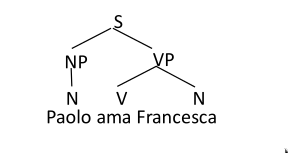
\includegraphics[scale=0.8]{01/sintassi.png}
  \end{center}
}

\dfn{Ambiguità}{
  Il linguaggio  naturale presenta frasi che possono essere interpretate in modi differenti.
}

\ex{Ambiguità}{
  \begin{center}
    "I made her duck"
  \end{center}

  \begin{itemize}
    \item Ho cucinato una papera per lei. 
    \item Ho cucinato una papera che apparteneva a lei. 
    \item Ho creato una papera con la stampante 3D e gliel'ho data a lei.
    \item Ho fatto abbassare la sua testa.
    \item In Harry Potter\footnote{Rowling merda.}: Ho trasformato lei in una papera.
  \end{itemize}
}

\clm{}{}{
  \begin{itemize}
    \item Le parole "duck" e "her" sono morfologicamente ambigue nella loro parte del discorso. "Duck" può essere un verbo o un nome, "her" può essere un pronome dativo o possessivo. 
    \item Il verbo "make" è sintetticamente ambiguo: può essere transitivo o intransitivo. 
    \item Inoltre "make" è anche semanticamente ambiguo: può significare creare o cucinare. 
    \item In una frase parlata c'è un altro livello per cui "her" può essere udito come "eye" e "make" come "maid".
  \end{itemize}
}

\nt{Essere ambigui permette di essere brevi e coincisi.}

\paragraph{Altre proprietà notevoli del linguaggio:}

\begin{itemize}
  \item Linguaggio non standard, evolve nel tempo. 
    \begin{itemize}
      \item Scialla bros $\rightarrow$ chill $\rightarrow$ è easy. 
      \begin{center}
    
\includegraphics[scale=0.5]{01/burns.png}
  \end{center}
    \end{itemize}
  \item Segmentazione. 
    \begin{itemize}
      \item Il treno Torino San Remo. 
    \end{itemize}
  \item Locuzioni, spesso l'interpretazione non è composizionale. 
    \begin{itemize}
      \item Pollica verde.
    \end{itemize}
  \item Neologismi. 
    \begin{itemize}
      \item Twettare\footnote{Musk merda.}
    \end{itemize}
  \item Conoscenza del mondo. 
    \begin{itemize}
      \item Lucia e Carola erano sorelle. 
      \item Lucia e Carola erano madri.
    \end{itemize}
  \item Meta-linguaggio. 
    \begin{itemize}
      \item La prima cosa bella ha avuto un
grandissimo successo.
    \end{itemize}
\end{itemize} 

\subsection{Lo Stato dell'Arte}

\begin{itemize}
  \item 1976: In Canada un sistema riesce a stampare due bollettini meteo in due lingue diverse. \item BabelFish, di Yahoo, era un sistema "a regole" di trascrizione automatica, basato su Systran.
  \item 2011: IBM costruisce un supercomputer per battere un essere umano a Jeopardy, Watson.  
  \item Tecnologie vocali: Speech Recognition, TextToSpeech, HTML5 Speech API (pagine web vocali).
\end{itemize}

\nt{
  Dopo sette milioni e mezzo di anni Pensiero Profondo fornisce la
  risposta: "42"\footnote{Guida Galattica per gli Autostoppisti.}. 
}

\begin{figure}[h]
    \centering
    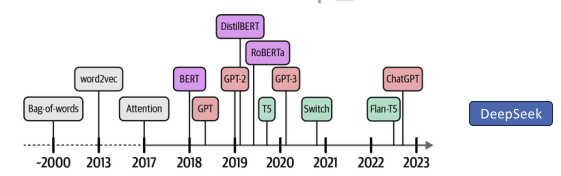
\includegraphics[scale=0.8]{01/timeline2.png}
    \caption{LLM. Tratto da "Hands-On Large Language Models", uscito nel Dicembre del 2024.}
\end{figure}

\nt{Well, Deepseek è open source e funziona meglio di ChatGPT (a patto che non chiedi cosa sia successo a piazza Tienanment nel 1989).}

\begin{figure}[h]
    \centering
    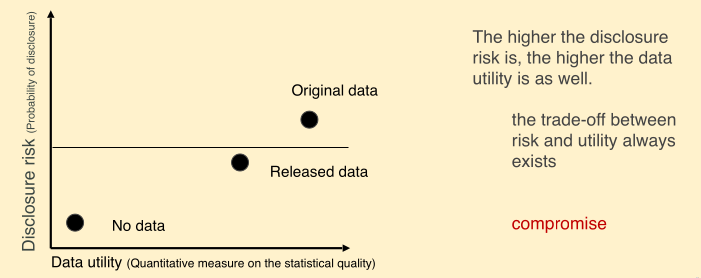
\includegraphics[scale=0.6]{01/data.png}
    \caption{Shifting di paradigma dovuto al Machine Learning.}
\end{figure}

\dfn{AI Generativa}{
  Modello di linguaggio di reti neurali multi-task basate sui transformer addestrati su una grande quantità di dati utilizzando self training e feedback umano.
}

\begin{itemize}
  \item Modello di Linguaggio: Text prediction $\rightarrow$ T9. 
  \item Multi-task: Google Translator, Siri.
\end{itemize}

\qs{}{Come fare un LLM (M. Lapata)?}

\begin{enumerate}
  \item Collezionare una grande quantità di dati. 
  \item Chiedere al LLM di predirre la nuova parola in una frase. 
  \item Ripetere il tutto.
\end{enumerate}

\begin{figure}[h]
    \centering
    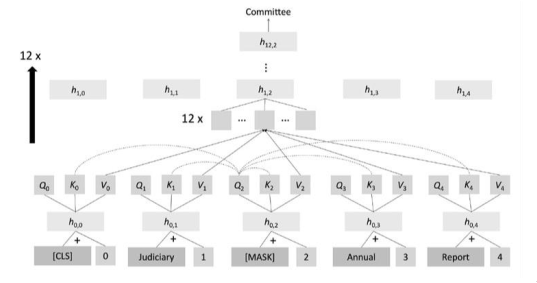
\includegraphics[scale=0.8]{01/addestramento.png}
    \caption{Auto addestramento di una rete neurale.}
\end{figure}

\qs{}{Come usare un LLM?}

\begin{itemize}
  \item Sintonizzazione a grana fine.
  \item Prompting.
\end{itemize}

\paragraph{Si può usare un LLM per:}

\begin{itemize}
  \item Search Engine. 
  \item Writer/Code assistant.
\end{itemize}

\nt{Noam Chomsky odia questi sistemi. Secondo lui servono per evitare l'apprendimento.}

\paragraph{DeepSeek:}

\begin{itemize}
  \item Apprendimento rinforzato automatico (senza essere umani). 
  \item Meno costoso $\rightarrow$ politicamente importante.
\end{itemize}

\paragraph{\fancyglitter{Il problema fondamentale}:} Convertire una frase o un testo in una forma che
permetta l'applicazione di meccanismi di
ragionamento automatico.

\section{I Livelli Linguistici}

\subsection{Da Frase a Significato}

\paragraph{Problema:} Convertire una frase o un testo in una forma che permetta l'applicazione di meccanismi di ragionamento automatico.

\begin{figure}[h]
    \centering
    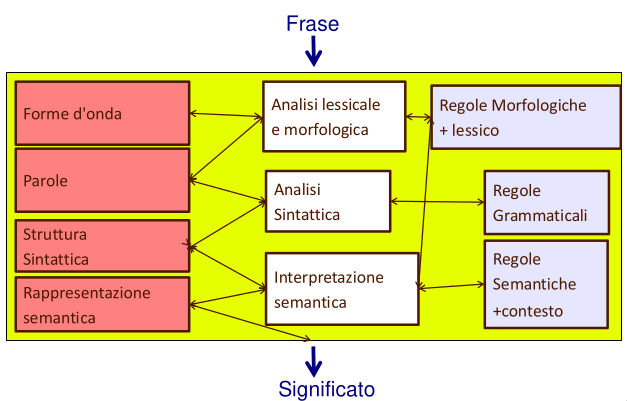
\includegraphics[scale=0.6]{01/fs.png}
    \caption{Passaggio da frase a significato.}
\end{figure}

\nt{Però la situazione non è così semplice. Bisogna capire come funzionano i moduli e come comunicano}

\paragraph{Nella linguistica computazionale c'è una divisione tra \fancyglitter{regole} e \fancyglitter{statistica}:}

\begin{itemize}
  \item Rules-driven. 
  \item Data-driven.
\end{itemize}

\nt{Steedman sostiene che i due aspetti dovrebberò convivere tra loro (2008). Evitare il regionamento tribale.}

\qs{}{Quando finisce una frase?}

\dfn{Sentence splitting}{
Task in cui si deve capire quando una frase finisce.
}

\begin{itemize}
  \item "!", "?" $\rightarrow$ Okay, pongono fine alla frase.
  \item ".":
    \begin{itemize}
      \item Fine frase. 
      \item Abbreviazione (Doc., Mx.). 
      \item Numeri (0.2).
    \end{itemize}
\end{itemize}

\qs{}{Quindi come si costruisce un classificatore binario che decida EoS (End of String) o not EoS?}

\begin{itemize}
  \item Si possono scrivere regole a mano: 
    \begin{itemize}
      \item Espressioni regolari. 
      \item Tokenizer (FA) e regole.
    \end{itemize}
  \item Addestrare un sistema di machine learning.
\end{itemize}

\begin{figure}[h]
    \centering
    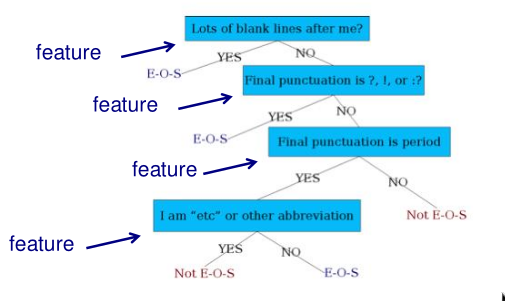
\includegraphics[scale=0.7]{01/decision tree.png}
    \caption{Albero di decisione.}
\end{figure}

\paragraph{Features più complesse:}

\begin{itemize}
  \item Caso di parole con ".".
  \item Caso di parole dopo ".". 
  \item Features numeriche: 
    \begin{itemize}
      \item Lunghezza di parole con ".". 
      \item Probabilità che una parola con "." avvenga alla fine della frase. 
      \item Probabilità che una parola dopo "." avvenga all'inizio di una frase.
    \end{itemize}
\end{itemize}

\qs{}{Cos'è davvero un albero di decisione?}

\begin{itemize}
  \item Una serie di IF-THEN-ELSE incapsulati. 
  \item Due possibilità per costruirlo: 
    \begin{itemize}
      \item \fancyglitter{By-hand}: solo in contesti semplici. 
      \item \fancyglitter{Machine learning}: su un training corpus.
    \end{itemize}
  \item Il punto cruciale è la scelta delle features.
\end{itemize}

\clm{}{}{
  \begin{itemize}
    \item In questo corso ci concentreremo sullo studio delle
feature linguistiche. 
\item In alcuni casi l'approccio by-hand verrà privilegiato poiché
è didatticamente più chiaro/semplice e poiché è più
semplice verificarne la fondatezza cognitiva mediante
introspezione.
  \end{itemize}
}

\qs{}{Nei sistemi end-to-end cosa sono le feature linguistiche?}

\dfn{Features Linguistiche Neurali}{
  L’architettura neurale, ovvero il numero e il tipo di
  connessioni, codifica in maniera \newfancyglitter{implicita} le features
linguistiche.
}

\nt{La ricerca, in questo caso, si focalizza su quale scelta
architetturale è più adatta alla modellazione implicita del
fenomeno linguistico e alla creazione del corpus di
training.}

\subsection{Il Livello Morfologico e l'Analisi Lessicale}

Il lessico è fondato sul concetto di \fancyglitter{parola}.

\qs{}{Che cos'è una parola?}

\begin{itemize}
  \item Intuitivamente è una
sequenza di caratteri delimitata da spazi o
punteggiatura. 
\item Sequenze di più parole, Es. passammela = passa a me essa. 
\item Le parole hanno un significato unitario (semantica
lessicale), ma volte sequenze di parole hanno un
significato unitario. Es. di corsa, by the way. 
\item In altre lingue il problema è più grave. 
  \begin{itemize}
    \item In tedesco: Lebenversicherungsgesellschaftangestellter = impiegato di una società di
assicurazione sulla vita. 
  \item In inglese: Wouldn't? = Would not.
  \end{itemize}
\end{itemize}

\paragraph{Presenza di suffissi:}

\begin{itemize}
  \item CAPITANO (forma non declinabile). 
  \item CAPITAN + O (nome o aggettivo o forma del verbo capitanare). 
  \item CAPIT + ANO (forma del verbo capitanare).
\end{itemize}

\begin{figure}[h]
    \centering
    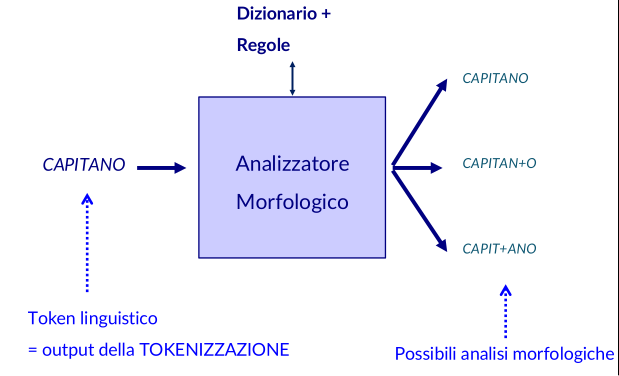
\includegraphics[scale=0.7]{01/analizzatore morfologico.png}
    \caption{Analizzatore morfologico.}
\end{figure}

\nt{Non c'è una forma giusta a priori, ma c'è una forma giusta in base al contesto.}

\dfn{Forme Composte}{
  Generalmente una parola contenuto più una (o più)
parole funzione.
}

\ex{Forme composte}{
  \paragraph{STAMPAMELO:}
  \begin{itemize}
    \item STAMP è una radice verbale. 
    \item A è un suffisso verbale. 
    \item ME e LO sono forme pronominali\footnote{Per triggerare gli Alt-Right.}.
  \end{itemize}
}

\dfn{Forme Multiple}{
  Le diversi componenti sono nel dizionario ma la
semantica non è composizionale.
}

\ex{Forme multiple}{
  \begin{itemize}
    \item Più o meno: puntatore tra le parole per recuperare la giusta semantica. 
    \item Prendere un abbaglio: rimandare all'interprete semantico.
  \end{itemize}
}

\dfn{Lemmatizzazione}{
  Trasformare un lemma in forma normale.
}

\nt{La forma normale non è stabile nel tempo.}

\dfn{Stemming}{
  Estrarre la forma radice (detta tema) da una parola.
}

\dfn{Paradigmatico}{Si cambia una parte della parola con una equivalente si ha una frase morfologicamente corretta.}

\dfn{Sintagmatico}{I rapporti che intercorrono tra gli elementi che si succedono nella frasei rapporti che intercorrono tra gli elementi che si succedono nella frase.}

\paragraph{Nome:}

\begin{itemize}
  \item Persone, oggetti, luoghi. 
  \item Proprietà sintagmatiche: 
    \begin{itemize}
      \item Comparire dopo gli articoli. 
      \item Avere un possessivo. 
      \item Avere un singolare o un plurale.
    \end{itemize}
  \item Comuni, propri, di massa, contabili.
\end{itemize}

\paragraph{Verbo:}

\begin{itemize}
  \item Eventi, azioni, processi. 
  \item Molte forme morfologiche. 
  \begin{itemize}
    \item Tempo. 
    \item Modo. 
    \item Numero.
  \end{itemize}
\item Tante categorie (ausiliari, modali, copula, etc.).
\end{itemize}

\paragraph{Aggettivi:}

\begin{itemize}
  \item Proprietà. 
\end{itemize}

\paragraph{Avverbi:}

\begin{itemize}
  \item Modificano qualcosa, spesso verbi, ma anche altri avverbi o intere frasi.
\end{itemize}

\nt{Nomi, verbi, aggettivi e avverbi sono \fancyglitter{di contenuto}, che puntano a oggetti reali.}

\dfn{Classi Aperte}{
  Classi che aumentano o scompaiono nel tempo costantemente (nomi, verbi, aggettivi, avverbi).
}

\dfn{Classi Chiuse}{
  Classi che aumentano o scompaiono con tempi lunghissimi.
}

\nt{Un esempio di classi chiuse sono i pronomi: una volta, in inglese, la seconda persona singolare era "thou", attualmente "you" ha assunto sia il ruolo di seconda persona singolare che plurale.}

\begin{figure}[h]
    \centering
    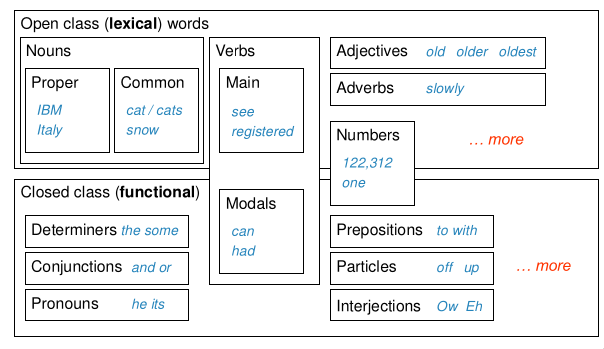
\includegraphics[scale=0.5]{01/opcl.png}
    \caption{Parti aperte e parti chiuse.}
\end{figure}

\paragraph{Google Unviversal PoS:} 12 PoS: NOUN (nouns), VERB (verbs), ADJ (adjectives), ADV (adverbs), PRON
(pronouns), DET (determiners and particles), ADP (prepositions and
postpositions), NUM (numerals), CONJ (conjunctions), PRT (particles), ‘.’
(punctuation marks) and X (a catch-all, e.g. abbreviations and foreign words). 

\subsection{Il Livello Sintattico}

\begin{figure}[h]
    \centering
    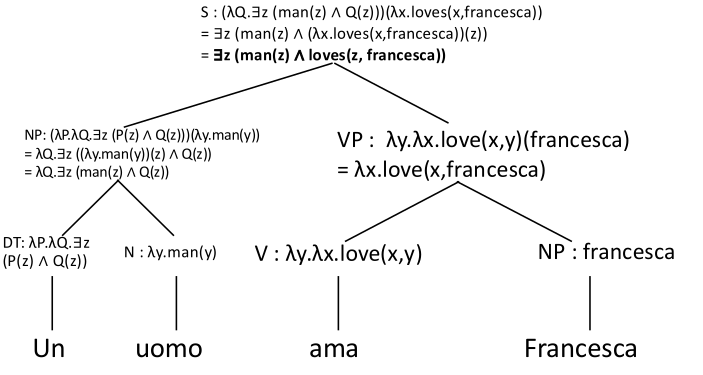
\includegraphics[scale=0.6]{01/paf.png}
    \caption{Parsing sintattico.}
\end{figure}

\nt{Le due alternative derivano da prospettive diverse: 
\begin{itemize}
  \item Quella a sinistra è la struttura sintagmatica (o a costituenti). 
  \item Quella a destra è la struttura a dipendenze (scuola di praga).
\end{itemize}
Entrambe le alternative sono equivalenti.
}

\dfn{Costituenza}{
  La struttura della frase organizza le parole in costituenti annidati.
}

\qs{}{
  Come si fa a sapere cos'è un costituente?
}

\begin{itemize}
  \item Distribuzione: un costituente si comporta come un'unità che compare in differenti parti della frase.
  \item Sostituzione: test per verificare un costituent 
\end{itemize}

\nt{La cosa interessante è automatizzare il processo della costruzione di alberi.}

\clm{}{}{
  \begin{itemize}
    \item NP:  la parola più importante sintatticamente è un nome.
    \item VP:  la parola più importante sintatticamente è un verbo.
    \item PP-LOC: la parola più importante sintatticamente è una preposizione.
  \end{itemize}
}

\begin{figure}[h]
    \centering
    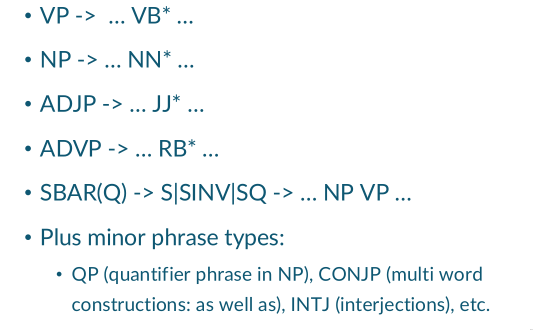
\includegraphics[scale=0.6]{01/struttura.png}
    \caption{Parti della sintassi.}
\end{figure}

\nt{I costituenti si comportano come un'unità:
\begin{itemize}
  \item Esperimento di Fodor-Bever. 
  \item Esperimento di Bock-Loebell.
\end{itemize}
}

\dfn{Context Free Grammar}{
  I CFG mettono in relazione i \newfancyglitter{simboli non terminali} e i \newfancyglitter{constituenti} (\textit{Chomsky}).
}

\dfn{X-barra}{
La teoria X-barra sostiene che se si costruisce un albero a costituenti con una determinata proprietà l'oggetto sarà presente internamente e il soggetto sarà presente esternamente.
}

\begin{figure}[h]
    \centering
    \includegraphics[scale=0.6]{01/X-barra}
    \caption{X-barra.}
\end{figure}

\dfn{Dipendenza}{
  Relazione tra due parole:
  \begin{itemize}
    \item \fancyglitter{Head}:  parola dominante.
    \item \fancyglitter{Dipendenza}:parola dominata.
  \end{itemize}
}

\nt{La testa seleziona le sue dipendenze e determina le loro proprietà.}

\cor{Argomenti}{
  Modificano in maniera sostanziale un evento (obbligatori).
}

\cor{Modificatori}{
  Modificano parzialmente un evento (facoltativi).
}

\subsection{Il Livello Semantico}

\paragraph{Esistono 2 approcci alla semantica lessicale:}

\begin{itemize}
  \item Classico. 
  \item Distribuzionale (anni '60): 
    \begin{itemize}
      \item Statistico. 
      \item Neurale.
    \end{itemize}
\end{itemize}

\dfn{Semantica Lessicale Classica}{
  Le connessioni sono legate al significato dei vari lessemi. La struttura interna dei lessemi è legata al significato.
}

\cor{Lessema}{
  Una coppia \newfancyglitter{forma-significato}, elemento del lessico.
}

\nt{Il problema è che sono possibili definizioni ricorsive "infinite".}

\paragraph{Relazioni tra lessemi:}

\begin{itemize}
  \item Omonimia: 2 lessemi con la stessa forma ortografica hanno due sensi diversi.
    \begin{itemize}
      \item A bank can hold the investments. 
      \item We can go on the right bank of the river.
    \end{itemize}
  \item Polisemia: lo stesso lessema ha due sensi diversi:
    \begin{itemize}
      \item A bank can hold the investments. 
      \item He got the blood from the bank.
    \end{itemize}
  \item Sinonimia: due lessemi con forma diversa hanno lo stesso senso (sostituibilità). 
    \begin{itemize}
      \item How big is that plane?
      \item How large is that plane?
    \end{itemize}
  \item Iponimia: due lessemi di cui uno denota una sottoclasse dell'altro: 
    \begin{itemize}
      \item Automobile è un iponimo di veicolo. 
      \item Veicolo è un iperonimo di automobile.
    \end{itemize}
\end{itemize}

\ex{Iponimia}{
  \begin{itemize}
    \item Quella è un automobile $\rightarrow$ quello è un veicolo. 
    \item (?) Quello è un veicolo $\rightarrow$ quella è un automobile.
  \end{itemize}
}

\cor{Syn-set}{
  Insieme di relazioni tra lessemi, usato per costruire le mappe in worldnet.
}

\dfn{Semantica Distribuzionale (vettoriale)}{
  Il significato di una parola è collegato alla distribuzione delle parole attorno a sé.
}

\ex{Semantica Distribuzionale}{
  \begin{itemize}
    \item A bottle of tesguino is on the table. 
    \item Everybody likes tesguino. 
    \item Tesguino makes you drunk.
  \end{itemize}
  Si può inferire che \textit{testguino} sia un super alcolico.
}

\paragraph{I vettori:}

\begin{itemize}
  \item Lunghi (lunghezza 20.000-50.000). 
  \item Sparsi (molti elementi sono zero).
\end{itemize}

\paragraph{I lean vectors:}

\begin{itemize}
  \item Piccoli (lunghezza 200-1000). 
  \item Densi (molti elementi sono non-zero). 
  \item Vettori più corti sono più facili da usare come feautures nel ML.
\end{itemize}

\begin{figure}[h]
    \centering
    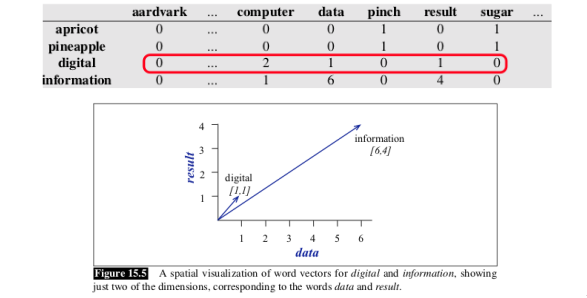
\includegraphics[scale=0.6]{01/occ.png}
    \caption{Si può andare a determinare la "vicinanza" di parole con la semantica vettoriale.}
\end{figure}

\clm{}{}{
  \begin{itemize}
    \item Con l'avvento delle reti neurali si ha un miglioramento. 
    \item vector(‘king’) - vector(‘man’) + vector(‘woman’) = vector(‘queen’). 
    \item vector(‘Paris’) - vector(‘France’) + vector(‘Italy’) = vector(‘Rome’).
  \end{itemize}
}

\dfn{Parole Contestualizzate}{
  Costruire un vettore per ogni parola, condizionandolo al suo contesto. La rappresentazione per ogni token è una funzione dell'intera sequenza di input.
}

\begin{figure}[h]
    \centering
    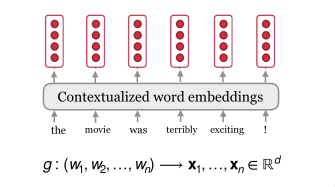
\includegraphics[scale=0.6]{01/context.png}
    \caption{Contestualizzazione.}
\end{figure}

\cor{Semantica Composizionale}{
  La semantica di un sintagma è funzione della semantica
dei sintagmi componenti; non dipende da altri sintagmi
esterni al sintagma stesso.
}

\nt{
  Conoscendo il significato di X, Y, e +, possiamo comporre
il significato “X+Y”.
}

\paragraph{Reasoning:}

\begin{itemize}
  \item Deduzione: conseguenza logica. 
  \item Induzione: basata su molti casi, si assume una regola generale. 
  \item Abduzione: regionamento per indizi.
\end{itemize}

\dfn{Metasemantica}{
  L'insieme di semantica composizionale e semantica lessicale distribuzionale. Serve per dare senso a parole sconosciute.
}

\subsection{Il Livello Pragmatico e del Discorso}

\dfn{Pragmatica}{L’interpretazione di “io” (sottinteso) e “oggi” dipende da
chi enuncia la frase e quando, rispettivamente.}

\nt{Il vero significato deve essere integrato da oggetti metalinguistici.}

\cor{Anafora}{
  Sintagmi che si riferiscono a oggetti
precedentemente menzionati.
}

\ex{Anafora}{
  \begin{itemize}
    \item “La torta era sul tavolo. Giorgio la divorò”. 
    \item “In giardino c’erano il cane e il gatto che giocavano con un
pezzo di stoffa. Il felino lacero’ la stoffa”.
    \item “Dopo essersi fidanzati, Giorgio e Maria trovarono un
prete e si sposarono. Per la luna di miele, essi andarono ai
Caraibi”.
  \end{itemize}
}

\paragraph{Le \fancyglitter{strutture dati} dei livelli:}

\begin{itemize}
  \item Livello morfologico e l'analisi lessicale: Lista. 
  \item Livello sintattico: Alberi. 
  \item Livello Semantico: 
    \begin{itemize}
      \item Semantica lessicale: Insiemi, Vettori. 
      \item Semantica formale: Logica, Alberi/Grafi. 
    \end{itemize}
  \item Livello paradigmatico e del discorso: Frame, Ontologie.
\end{itemize}




